\documentclass{standalone}
\usepackage{tikz}
\usetikzlibrary{patterns, positioning}


\begin{document}
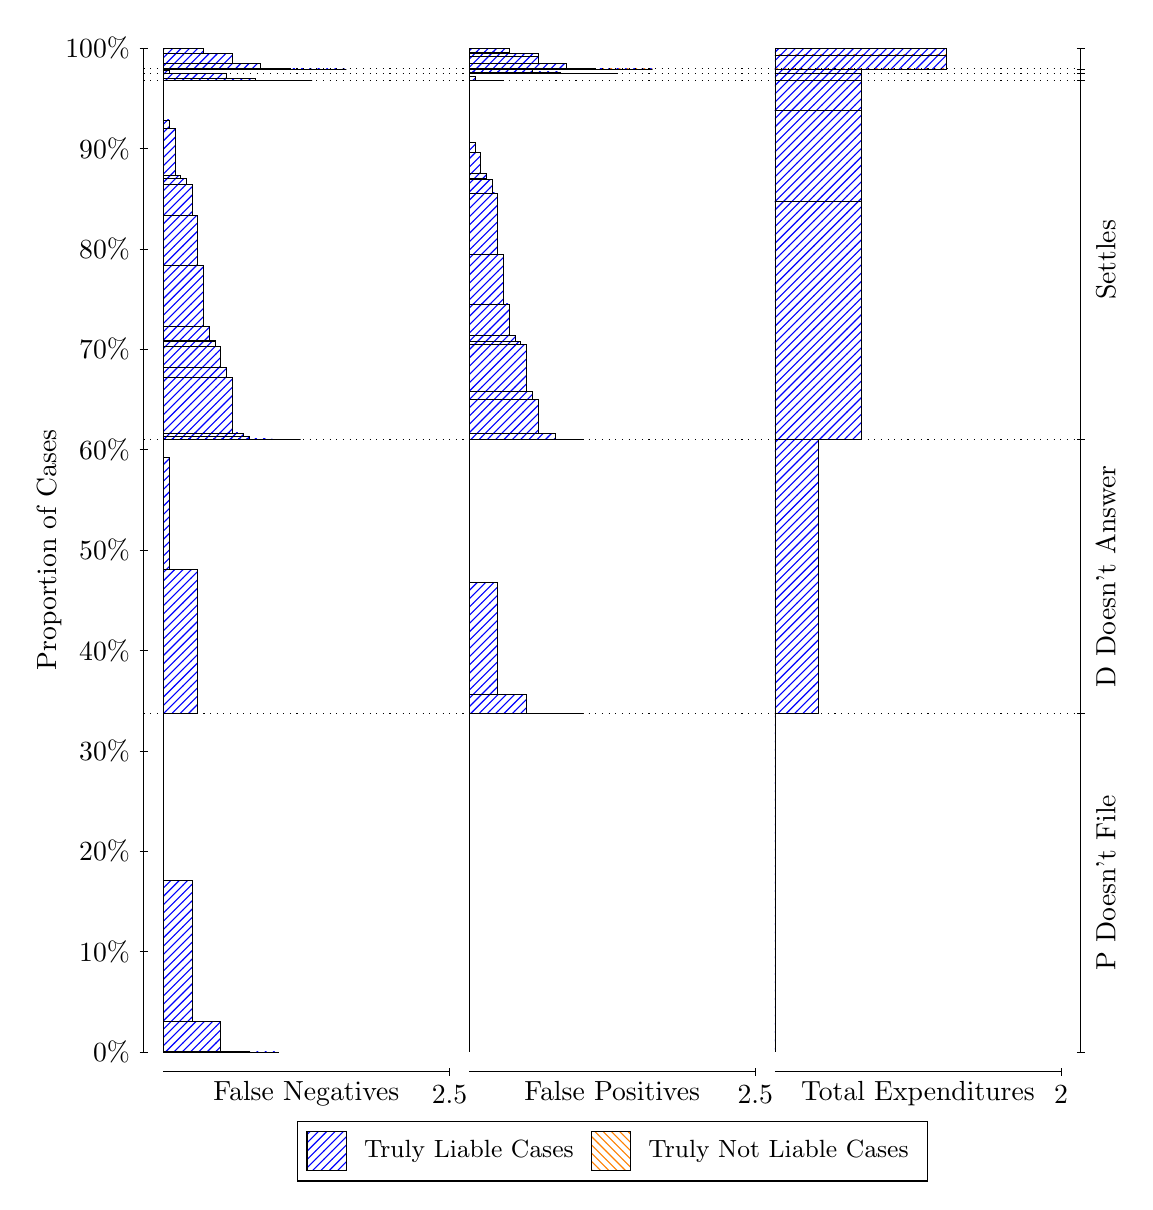
\begin{tikzpicture}
\draw[black, very thin] (1.5,1.75) -- (1.5,14.5);
\node[rotate=90, text=black, anchor=center] at (0.3, 8.125) {Proportion of Cases};
\draw[black, very thin] (1.45,1.75) -- (1.55,1.75);
\node[text=black, anchor=east] at (1.45, 1.75) {0\%};
\draw[black, very thin] (1.45,3.025) -- (1.55,3.025);
\node[text=black, anchor=east] at (1.45, 3.025) {10\%};
\draw[black, very thin] (1.45,4.3) -- (1.55,4.3);
\node[text=black, anchor=east] at (1.45, 4.3) {20\%};
\draw[black, very thin] (1.45,5.575) -- (1.55,5.575);
\node[text=black, anchor=east] at (1.45, 5.575) {30\%};
\draw[black, very thin] (1.45,6.85) -- (1.55,6.85);
\node[text=black, anchor=east] at (1.45, 6.85) {40\%};
\draw[black, very thin] (1.45,8.125) -- (1.55,8.125);
\node[text=black, anchor=east] at (1.45, 8.125) {50\%};
\draw[black, very thin] (1.45,9.4) -- (1.55,9.4);
\node[text=black, anchor=east] at (1.45, 9.4) {60\%};
\draw[black, very thin] (1.45,10.675) -- (1.55,10.675);
\node[text=black, anchor=east] at (1.45, 10.675) {70\%};
\draw[black, very thin] (1.45,11.95) -- (1.55,11.95);
\node[text=black, anchor=east] at (1.45, 11.95) {80\%};
\draw[black, very thin] (1.45,13.225) -- (1.55,13.225);
\node[text=black, anchor=east] at (1.45, 13.225) {90\%};
\draw[black, very thin] (1.45,14.5) -- (1.55,14.5);
\node[text=black, anchor=east] at (1.45, 14.5) {100\%};

\draw[black, very thin] (13.4,1.75) -- (13.4,14.5);
\draw[black, very thin] (13.35,1.75) -- (13.45,1.75);
\node[anchor=west] at (13.35, 1.75) {};
\draw[black, very thin] (13.35,6.051) -- (13.45,6.051);
\node[anchor=west] at (13.35, 6.051) {};
\draw[black, very thin] (13.35,9.5338) -- (13.45,9.5338);
\node[anchor=west] at (13.35, 9.5338) {};
\draw[black, very thin] (13.35,14.086) -- (13.45,14.086);
\node[anchor=west] at (13.35, 14.086) {};
\draw[black, very thin] (13.35,14.174) -- (13.45,14.174);
\node[anchor=west] at (13.35, 14.174) {};
\draw[black, very thin] (13.35,14.236) -- (13.45,14.236);
\node[anchor=west] at (13.35, 14.236) {};
\draw[black, very thin] (13.35,14.5) -- (13.45,14.5);
\node[anchor=west] at (13.35, 14.5) {};

\draw[black, very thin, pattern color=blue, pattern=north east lines] (1.75,1.75) rectangle (3.2033,1.7501);
\draw[black, very thin, pattern color=blue, pattern=north east lines] (1.75,1.7501) rectangle (2.84,1.7611);
\draw[black, very thin, pattern color=blue, pattern=north east lines] (1.75,1.7611) rectangle (2.4767,2.1337);
\draw[black, very thin, pattern color=blue, pattern=north east lines] (1.75,2.1337) rectangle (2.1133,3.9293);
\draw[black, very thin, pattern color=orange, pattern=north west lines] (1.75,3.9293) rectangle (1.75,3.9293);
\draw[black, very thin, pattern color=blue, pattern=north east lines] (1.75,3.9293) rectangle (1.75,6.051);
\draw[black, very thin, pattern color=blue, pattern=north east lines] (1.75,6.051) rectangle (2.186,7.8739);
\draw[black, very thin, pattern color=blue, pattern=north east lines] (1.75,7.8739) rectangle (1.8227,9.2977);
\draw[black, very thin, pattern color=orange, pattern=north west lines] (1.75,9.2977) rectangle (1.75,9.2977);
\draw[black, very thin, pattern color=blue, pattern=north east lines] (1.75,9.2977) rectangle (1.75,9.5338);
\draw[black, very thin, pattern color=blue, pattern=north east lines] (1.75,9.5338) rectangle (3.494,9.5338);
\draw[black, very thin, pattern color=blue, pattern=north east lines] (1.75,9.5338) rectangle (3.2033,9.5339);
\draw[black, very thin, pattern color=blue, pattern=north east lines] (1.75,9.5339) rectangle (3.1307,9.5348);
\draw[black, very thin, pattern color=blue, pattern=north east lines] (1.75,9.5348) rectangle (3.058,9.5348);
\draw[black, very thin, pattern color=blue, pattern=north east lines] (1.75,9.5348) rectangle (2.9127,9.5352);
\draw[black, very thin, pattern color=blue, pattern=north east lines] (1.75,9.5352) rectangle (2.84,9.566);
\draw[black, very thin, pattern color=blue, pattern=north east lines] (1.75,9.566) rectangle (2.7673,9.6031);
\draw[black, very thin, pattern color=blue, pattern=north east lines] (1.75,9.6031) rectangle (2.6947,9.6111);
\draw[black, very thin, pattern color=blue, pattern=north east lines] (1.75,9.6111) rectangle (2.622,10.322);
\draw[black, very thin, pattern color=blue, pattern=north east lines] (1.75,10.322) rectangle (2.5493,10.443);
\draw[black, very thin, pattern color=blue, pattern=north east lines] (1.75,10.443) rectangle (2.4767,10.709);
\draw[black, very thin, pattern color=blue, pattern=north east lines] (1.75,10.709) rectangle (2.404,10.78);
\draw[black, very thin, pattern color=blue, pattern=north east lines] (1.75,10.78) rectangle (2.404,10.788);
\draw[black, very thin, pattern color=blue, pattern=north east lines] (1.75,10.788) rectangle (2.3313,10.96);
\draw[black, very thin, pattern color=blue, pattern=north east lines] (1.75,10.96) rectangle (2.2587,11.739);
\draw[black, very thin, pattern color=blue, pattern=north east lines] (1.75,11.739) rectangle (2.186,12.37);
\draw[black, very thin, pattern color=blue, pattern=north east lines] (1.75,12.37) rectangle (2.1133,12.772);
\draw[black, very thin, pattern color=blue, pattern=north east lines] (1.75,12.772) rectangle (2.0407,12.846);
\draw[black, very thin, pattern color=blue, pattern=north east lines] (1.75,12.846) rectangle (2.0407,12.846);
\draw[black, very thin, pattern color=blue, pattern=north east lines] (1.75,12.846) rectangle (1.968,12.882);
\draw[black, very thin, pattern color=blue, pattern=north east lines] (1.75,12.882) rectangle (1.8953,13.48);
\draw[black, very thin, pattern color=blue, pattern=north east lines] (1.75,13.48) rectangle (1.8227,13.586);
\draw[black, very thin, pattern color=orange, pattern=north west lines] (1.75,13.586) rectangle (1.75,13.586);
\draw[black, very thin, pattern color=blue, pattern=north east lines] (1.75,13.586) rectangle (1.75,14.086);
\draw[black, very thin, pattern color=blue, pattern=north east lines] (1.75,14.086) rectangle (3.6393,14.086);
\draw[black, very thin, pattern color=blue, pattern=north east lines] (1.75,14.086) rectangle (3.276,14.086);
\draw[black, very thin, pattern color=blue, pattern=north east lines] (1.75,14.086) rectangle (2.9127,14.119);
\draw[black, very thin, pattern color=blue, pattern=north east lines] (1.75,14.119) rectangle (2.5493,14.173);
\draw[black, very thin, pattern color=blue, pattern=north east lines] (1.75,14.173) rectangle (2.186,14.174);
\draw[black, very thin, pattern color=orange, pattern=north west lines] (1.75,14.174) rectangle (1.75,14.174);
\draw[black, very thin, pattern color=blue, pattern=north east lines] (1.75,14.174) rectangle (2.186,14.175);
\draw[black, very thin, pattern color=blue, pattern=north east lines] (1.75,14.175) rectangle (1.8227,14.213);
\draw[black, very thin, pattern color=orange, pattern=north west lines] (1.75,14.213) rectangle (1.75,14.213);
\draw[black, very thin, pattern color=blue, pattern=north east lines] (1.75,14.213) rectangle (1.75,14.236);
\draw[black, very thin, pattern color=blue, pattern=north east lines] (1.75,14.236) rectangle (4.0753,14.236);
\draw[black, very thin, pattern color=blue, pattern=north east lines] (1.75,14.236) rectangle (3.712,14.236);
\draw[black, very thin, pattern color=blue, pattern=north east lines] (1.75,14.236) rectangle (3.3487,14.241);
\draw[black, very thin, pattern color=blue, pattern=north east lines] (1.75,14.241) rectangle (2.9853,14.302);
\draw[black, very thin, pattern color=blue, pattern=north east lines] (1.75,14.302) rectangle (2.622,14.434);
\draw[black, very thin, pattern color=blue, pattern=north east lines] (1.75,14.434) rectangle (2.2587,14.496);
\draw[black, very thin, pattern color=blue, pattern=north east lines] (1.75,14.496) rectangle (1.8953,14.5);
\draw[black, very thin, pattern color=orange, pattern=north west lines] (1.75,14.5) rectangle (1.75,14.5);
\draw[black, very thin, pattern color=blue, pattern=north east lines] (1.75,14.5) rectangle (1.75,14.5);
\draw[black, very thin, pattern color=orange, pattern=north west lines] (5.6333,1.75) rectangle (5.6333,1.75);
\draw[black, very thin, pattern color=blue, pattern=north east lines] (5.6333,1.75) rectangle (5.6333,6.051);
\draw[black, very thin, pattern color=orange, pattern=north west lines] (5.6333,6.051) rectangle (7.0867,6.051);
\draw[black, very thin, pattern color=blue, pattern=north east lines] (5.6333,6.051) rectangle (7.0867,6.051);
\draw[black, very thin, pattern color=blue, pattern=north east lines] (5.6333,6.051) rectangle (6.7233,6.0521);
\draw[black, very thin, pattern color=blue, pattern=north east lines] (5.6333,6.0521) rectangle (6.36,6.2871);
\draw[black, very thin, pattern color=blue, pattern=north east lines] (5.6333,6.2871) rectangle (5.9967,7.7109);
\draw[black, very thin, pattern color=blue, pattern=north east lines] (5.6333,7.7109) rectangle (5.6333,9.5338);
\draw[black, very thin, pattern color=orange, pattern=north west lines] (5.6333,9.5338) rectangle (7.0867,9.5338);
\draw[black, very thin, pattern color=blue, pattern=north east lines] (5.6333,9.5338) rectangle (7.0867,9.5339);
\draw[black, very thin, pattern color=orange, pattern=north west lines] (5.6333,9.5339) rectangle (6.9413,9.5339);
\draw[black, very thin, pattern color=blue, pattern=north east lines] (5.6333,9.5339) rectangle (6.9413,9.5339);
\draw[black, very thin, pattern color=orange, pattern=north west lines] (5.6333,9.5339) rectangle (6.796,9.5339);
\draw[black, very thin, pattern color=blue, pattern=north east lines] (5.6333,9.5339) rectangle (6.796,9.5343);
\draw[black, very thin, pattern color=blue, pattern=north east lines] (5.6333,9.5343) rectangle (6.7233,9.6062);
\draw[black, very thin, pattern color=orange, pattern=north west lines] (5.6333,9.6062) rectangle (6.6507,9.6062);
\draw[black, very thin, pattern color=blue, pattern=north east lines] (5.6333,9.6062) rectangle (6.6507,9.6066);
\draw[black, very thin, pattern color=blue, pattern=north east lines] (5.6333,9.6066) rectangle (6.578,9.6093);
\draw[black, very thin, pattern color=orange, pattern=north west lines] (5.6333,9.6093) rectangle (6.5053,9.6093);
\draw[black, very thin, pattern color=blue, pattern=north east lines] (5.6333,9.6093) rectangle (6.5053,10.034);
\draw[black, very thin, pattern color=blue, pattern=north east lines] (5.6333,10.034) rectangle (6.4327,10.14);
\draw[black, very thin, pattern color=blue, pattern=north east lines] (5.6333,10.14) rectangle (6.36,10.737);
\draw[black, very thin, pattern color=blue, pattern=north east lines] (5.6333,10.737) rectangle (6.2873,10.774);
\draw[black, very thin, pattern color=orange, pattern=north west lines] (5.6333,10.774) rectangle (6.2147,10.774);
\draw[black, very thin, pattern color=blue, pattern=north east lines] (5.6333,10.774) rectangle (6.2147,10.774);
\draw[black, very thin, pattern color=blue, pattern=north east lines] (5.6333,10.774) rectangle (6.2147,10.848);
\draw[black, very thin, pattern color=blue, pattern=north east lines] (5.6333,10.848) rectangle (6.142,11.25);
\draw[black, very thin, pattern color=blue, pattern=north east lines] (5.6333,11.25) rectangle (6.0693,11.88);
\draw[black, very thin, pattern color=blue, pattern=north east lines] (5.6333,11.88) rectangle (5.9967,12.66);
\draw[black, very thin, pattern color=blue, pattern=north east lines] (5.6333,12.66) rectangle (5.924,12.832);
\draw[black, very thin, pattern color=blue, pattern=north east lines] (5.6333,12.832) rectangle (5.8513,12.84);
\draw[black, very thin, pattern color=blue, pattern=north east lines] (5.6333,12.84) rectangle (5.8513,12.911);
\draw[black, very thin, pattern color=blue, pattern=north east lines] (5.6333,12.911) rectangle (5.7787,13.177);
\draw[black, very thin, pattern color=blue, pattern=north east lines] (5.6333,13.177) rectangle (5.706,13.298);
\draw[black, very thin, pattern color=blue, pattern=north east lines] (5.6333,13.298) rectangle (5.6333,14.086);
\draw[black, very thin, pattern color=orange, pattern=north west lines] (5.6333,14.086) rectangle (6.0693,14.086);
\draw[black, very thin, pattern color=blue, pattern=north east lines] (5.6333,14.086) rectangle (6.0693,14.087);
\draw[black, very thin, pattern color=blue, pattern=north east lines] (5.6333,14.087) rectangle (5.706,14.141);
\draw[black, very thin, pattern color=blue, pattern=north east lines] (5.6333,14.141) rectangle (5.6333,14.174);
\draw[black, very thin, pattern color=orange, pattern=north west lines] (5.6333,14.174) rectangle (7.5227,14.174);
\draw[black, very thin, pattern color=blue, pattern=north east lines] (5.6333,14.174) rectangle (7.5227,14.174);
\draw[black, very thin, pattern color=blue, pattern=north east lines] (5.6333,14.174) rectangle (7.1593,14.175);
\draw[black, very thin, pattern color=blue, pattern=north east lines] (5.6333,14.175) rectangle (6.796,14.198);
\draw[black, very thin, pattern color=blue, pattern=north east lines] (5.6333,14.198) rectangle (6.4327,14.236);
\draw[black, very thin, pattern color=blue, pattern=north east lines] (5.6333,14.236) rectangle (6.0693,14.236);
\draw[black, very thin, pattern color=orange, pattern=north west lines] (5.6333,14.236) rectangle (7.9587,14.236);
\draw[black, very thin, pattern color=blue, pattern=north east lines] (5.6333,14.236) rectangle (7.9587,14.236);
\draw[black, very thin, pattern color=orange, pattern=north west lines] (5.6333,14.236) rectangle (7.5953,14.236);
\draw[black, very thin, pattern color=blue, pattern=north east lines] (5.6333,14.236) rectangle (7.5953,14.236);
\draw[black, very thin, pattern color=orange, pattern=north west lines] (5.6333,14.236) rectangle (7.232,14.236);
\draw[black, very thin, pattern color=blue, pattern=north east lines] (5.6333,14.236) rectangle (7.232,14.241);
\draw[black, very thin, pattern color=blue, pattern=north east lines] (5.6333,14.241) rectangle (6.8687,14.302);
\draw[black, very thin, pattern color=orange, pattern=north west lines] (5.6333,14.302) rectangle (6.8687,14.302);
\draw[black, very thin, pattern color=blue, pattern=north east lines] (5.6333,14.302) rectangle (6.8687,14.302);
\draw[black, very thin, pattern color=blue, pattern=north east lines] (5.6333,14.302) rectangle (6.5053,14.397);
\draw[black, very thin, pattern color=orange, pattern=north west lines] (5.6333,14.397) rectangle (6.5053,14.397);
\draw[black, very thin, pattern color=blue, pattern=north east lines] (5.6333,14.397) rectangle (6.5053,14.435);
\draw[black, very thin, pattern color=blue, pattern=north east lines] (5.6333,14.435) rectangle (6.142,14.45);
\draw[black, very thin, pattern color=blue, pattern=north east lines] (5.6333,14.45) rectangle (6.142,14.496);
\draw[black, very thin, pattern color=blue, pattern=north east lines] (5.6333,14.496) rectangle (5.7787,14.496);
\draw[black, very thin, pattern color=blue, pattern=north east lines] (5.6333,14.496) rectangle (5.7787,14.5);
\draw[black, very thin, pattern color=blue, pattern=north east lines] (5.6333,14.5) rectangle (5.6333,14.5);
\draw[black, very thin, pattern color=orange, pattern=north west lines] (9.5167,1.75) rectangle (9.5167,1.75);
\draw[black, very thin, pattern color=blue, pattern=north east lines] (9.5167,1.75) rectangle (9.5167,6.051);
\draw[black, very thin, pattern color=orange, pattern=north west lines] (9.5167,6.051) rectangle (10.062,6.051);
\draw[black, very thin, pattern color=blue, pattern=north east lines] (9.5167,6.051) rectangle (10.062,9.5338);
\draw[black, very thin, pattern color=orange, pattern=north west lines] (9.5167,9.5338) rectangle (10.607,9.5338);
\draw[black, very thin, pattern color=blue, pattern=north east lines] (9.5167,9.5338) rectangle (10.607,12.553);
\draw[black, very thin, pattern color=orange, pattern=north west lines] (9.5167,12.553) rectangle (10.607,12.553);
\draw[black, very thin, pattern color=blue, pattern=north east lines] (9.5167,12.553) rectangle (10.607,13.709);
\draw[black, very thin, pattern color=orange, pattern=north west lines] (9.5167,13.709) rectangle (10.607,13.709);
\draw[black, very thin, pattern color=blue, pattern=north east lines] (9.5167,13.709) rectangle (10.607,14.086);
\draw[black, very thin, pattern color=orange, pattern=north west lines] (9.5167,14.086) rectangle (10.607,14.086);
\draw[black, very thin, pattern color=blue, pattern=north east lines] (9.5167,14.086) rectangle (10.607,14.174);
\draw[black, very thin, pattern color=orange, pattern=north west lines] (9.5167,14.174) rectangle (10.607,14.174);
\draw[black, very thin, pattern color=blue, pattern=north east lines] (9.5167,14.174) rectangle (10.607,14.236);
\draw[black, very thin, pattern color=orange, pattern=north west lines] (9.5167,14.236) rectangle (11.697,14.236);
\draw[black, very thin, pattern color=blue, pattern=north east lines] (9.5167,14.236) rectangle (11.697,14.412);
\draw[black, very thin, pattern color=orange, pattern=north west lines] (9.5167,14.412) rectangle (11.697,14.412);
\draw[black, very thin, pattern color=blue, pattern=north east lines] (9.5167,14.412) rectangle (11.697,14.5);
\draw[black, dotted] (1.5,6.051) -- (13.4,6.051);
\draw[black, dotted] (1.5,9.5338) -- (13.4,9.5338);
\draw[black, dotted] (1.5,14.086) -- (13.4,14.086);
\draw[black, dotted] (1.5,14.174) -- (13.4,14.174);
\draw[black, dotted] (1.5,14.236) -- (13.4,14.236);
\draw[black, very thin] (1.75,1.5) -- (5.3833,1.5);
\node[text=black, anchor=north] at (3.5667, 1.5) {False Negatives};
\draw[black, very thin] (5.3833,1.45) -- (5.3833,1.55);
\node[text=black, anchor=north] at (5.3833, 1.45) {2.5};

\draw[black, very thin] (5.6333,1.5) -- (9.2667,1.5);
\node[text=black, anchor=north] at (7.45, 1.5) {False Positives};
\draw[black, very thin] (9.2667,1.45) -- (9.2667,1.55);
\node[text=black, anchor=north] at (9.2667, 1.45) {2.5};

\draw[black, very thin] (9.5167,1.5) -- (13.15,1.5);
\node[text=black, anchor=north] at (11.333, 1.5) {Total Expenditures};
\draw[black, very thin] (13.15,1.45) -- (13.15,1.55);
\node[text=black, anchor=north] at (13.15, 1.45) {2};

\node[text=black, centered, rotate=90] at (13.72, 3.9005) {P Doesn't File};
\node[text=black, centered, rotate=90] at (13.72, 7.7924) {D Doesn't Answer};
\node[text=black, centered, rotate=90] at (13.72, 11.81) {Settles};




\draw (7.449999999999999,1.5) node[draw=none] (baseCoordinate) {};
\begin{scope}[align=center]
        \matrix[scale=0.5, draw=black, below=0.5cm of baseCoordinate, nodes={draw}, column sep=0.1cm]{
            \node[rectangle, draw, minimum width=0.5cm, minimum height=0.5cm, pattern color=blue, pattern=north east lines] {}; &
            \node[draw=none, font=\small, text=black] (B) {Truly Liable Cases}; &
            \node[rectangle, draw, minimum width=0.5cm, minimum height=0.5cm, pattern color=orange, pattern=north west lines] {}; &
            \node[draw=none, font=\small, text=black] (B) {Truly Not Liable Cases}; \\
            };
\end{scope}

\end{tikzpicture}
\end{document}